% EIC digitisation writeup

%\documentclass[a4paper,11pt,twocolumn]{article}
\documentclass[CP]{copernicus}
\usepackage[pdftex]{graphicx}
%\usepackage{lineno}

\begin{document}
\title{Recovering climate records for 1789--1834 from English-East-India Company ship's logs}

\runningauthor{BROHAN ET AL}
% Author names in capital letters,
\runningtitle{EEIC CLIMATE RECORDS 1789-1834 - DRAFT 2}
% Shorter version of title entered in capital letters

\author[1]{Philip Brohan}
\author[1]{Rob Allan}
\author[2]{Eric Freeman}
\author[3]{Dennis Wheeler}
\author[4]{Clive Wilkinson}
\author[3,4]{Fiona Williamson}
\date{Draft 2 --- 13 July 2011}

\affil[1]{Met Office Hadley Centre, Exeter, UK.}
\affil[2]{NOAA/STG Inc., USA}
\affil[3]{Sunderland University, Sunderland, UK}
\affil[4]{University of East Anglia, Norwich, UK}

\correspondence{Philip Brohan\\ (philip.brohan@metoffice.gov.uk)}
\firstpage{1}

\maketitle

\begin{abstract}

Although large-scale systematic collection of surface marine weather observations by meteorological agencies started after 1853, with the Brussels conference organised by Matthew Maury; mariners were making and recording observations long before. One organisation which systematically made observations and collected the results was the English East-India Company (EEIC), and their archives have been preserved in the British Library. Inspection of those archives revealed 900 log-books of EEIC ships containing daily instrumental measurements of temperature and pressure, and subjective estimates of wind speed and direction, from voyages across the Atlantic and Indian Ocean between 1789 and 1834. Those records have been extracted and digitised, providing nearly 300,000 new weather records offering an unprecedentedly detailed view of the weather and climate of the late eighteenth and early nineteenth centuries.
\end{abstract}

\introduction

Amongst the archives in the British Library (BL) in London are some 4000 logbooks from ships in the service of the English East India Company (EEIC); each recording the details and events of a voyage from England to the Indies (usually India, China or both) and back, typically taking the best part of two years. The EEIC received its charter from Elizabeth I in 1600, and many of its earliest voyages became famous because of their excellent records of new lands; for example that by Henry Middleton to the Moluccas in 1604-6 \citep{Foster10}. These early voyages were recorded in diaries; logbooks --- formally prepared documents of a standard format --- did not begin to appear until the 1650s. Their preparation was part of an officer's duties until the gradual expansion of the Company in the 1830s into a quasi-military and political body responsible for overseeing British interests in India and beyond. Those archived in the BL, therefore, extend from the 1600s through to the 1830s, and are well known to historians \citep{Farrington99}: They document social conditions, discipline, medicine and health, the trade and transport of goods, people and passengers. They touch on first contact with new lands and peoples, convey colonial attitudes and cultures, and describe long lost coastal towns and villages. Many even contain detailed drawings of coastlines, ships, mammals, birds and sea creatures.    

Ship's logbooks are also valuable sources of historical climate data (\citet{chenoweth96,wheeler06cliwoc,brohan09digitisation,brohan10corral}), and the EEIC logbooks include daily records of the weather along the routes taken by the ships: They cover large parts of the Atlantic and Indian Oceans, and include the occasional foray into the Pacific. All the logbooks contain wind speed and direction records, as this was vital information for early navigators, but the later logs, starting in about 1790, are even more valuable, as some of them contain daily thermometer and barometer observations as well as the wind reports. The principal instigator of the addition of instrumental observations was Alexander Dalrymple --- the Company's, and later the Royal Navy's, first hydrographer {\bf[reference for Dalyrmple]}. Dalrymple was both an explorer and an enthusiastic scientist, and, as hydrographer, he was responsible for ensuring that the EEIC ships could transport goods to and from England as quickly as possible and at minimum risk of loss. With this in mind, he equipped the East Indiaman Grenville with a set of meteorological instruments for her voyage in 1775 under Captain Burnet Abercrombie \citep{Dalrymple78}, and set a pattern to be later adopted by all EEIC officers. 

It is the routine inclusion of regular instrumental weather observations that distinguishes the EEIC logbooks from all of their contemporaries such as the Royal Navy and the Hudson's Bay Company (which did not routinely make such records until many years later). The EEIC logbook records offer a potential source of detailed information on climate change and variability over a large area of tropical and sub-tropical ocean for the late eighteenth and early nineteenth century - a time and region where other observations are almost completely missing. About 10\% of these logbook observations have been examined in previous studies \citep{chenoweth96,farrington98,chenoweth00homogenization}, but most of them have never been digitised or examined, and none have made it into the standard climate datasets for widespread use. This paper discusses a project to find and digitise all the instrumental (thermometer and barometer) observations from this source. The digitised observations are attached as supplementary information, and have been submitted to the International Comprehensive Ocean-Atmosphere Dataset (ICOADS, \citet{woodruff11icoads}) for inclusion in future versions.

\section{Digitisation of the weather records}

The British Library's EEIC logbook collection has been catalogued \citep{Farrington99}, but that catalogue, though extensive, does not distinguish those logbooks that contain instrumental data. So research was undertaken in the British Library archives to produce a catalogue detailing exactly which logs contain instrumental observations; whether the observations are of pressure, air or sea surface temperature; the name of the ship; the year of its voyage; and the ship's route with dates. It also includes additional information such as how frequently the readings were taken, and whether any unusual weather events took place. In the event almost all of the logbooks dating from 1790 or later contained some instrumental observations, but not every log contained observations, and on occasion observational records were sporadic.  {\bf[We should include this catalogue as supplementary information]}.

Using this catalogue, the 891 logbooks including consistent instrumental records were selected for digitisation: the earliest that of the Melville Castle, starting in February 1789; and the last that of the Sherborne, finishing in August 1834. Figure \ref{Ftl1} shows a typical example, logbook records for one day from EIC ship Carmarthen.
\begin{figure*}[!hbp]
\begin{center}
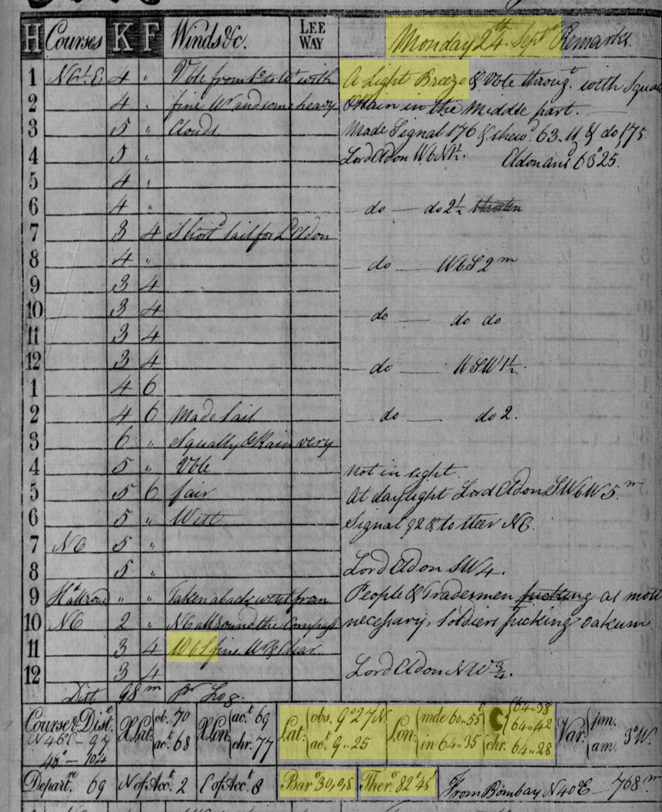
\includegraphics[angle=0, width=0.8\textwidth]{../figures/logbook_Carmarthen_Sept_24_1810+highlights}
\caption{Logbook of EIC ship Carmarthen for 24th September 1810. Ship's days run from noon to noon 12 hours ahead of the civil day, so this covers the afternoon of the 23rd and the morning of the 24th. For each hour there is space to enter the ship's course, its speed (in Knots and Fathoms), and the wind direction. To the right of this table is a section for general remarks (which almost always includes reference to the wind speed); and at the bottom is a table of summary data for the day. The elements digitised are highlighted in yellow. from top to bottom they are: the date (September 24th); the wind force (a light breeze --- Beaufort force 2), the wind direction (West by South - $258.75^\circ$ magnetic), the noon position (9 degrees 27 minutes North, 64 degrees 28 minutes East), the barometric pressure (30.05 inches of mercury) and the air temperature (82 degrees 45 minutes --- $82.75^\circ$ Fahrenheit).}
\label{Ftl1}
\end{center}
\end{figure*}
That logbook records a voyage from London to Bombay, and back to the UK, through the Atlantic and Indian Oceans, and round the Cape of Good Hope. The voyage took 20 months (May 1810 to January 1812); records were only made on days when the ship was at sea, but even so the logbook includes 372 such daily records.

Digitising each day's observations from all 891 logbooks proved to be a major undertaking. To make it possible to work on the logbooks outside the BL, the books were photographed. This produced about 140,000 digital images, each showing one page. Most pages contained two day's records on a standard pre-printed form (figure \ref{Ftl1} shows the top half of one page) though, in rare cases, variant form types were used that only containted one day's records; also hand-drawn forms were occasionally used --- presumably to make up a shortfall in printed forms. These images were indexed and stored in the electronic media archive of the U.S. Climate Database Modernisation Program (CDMP), managed from the National Oceanic and Atmospheric administration's (NOAA) National Climatic Data Center (NCDC). CDMP's mandate is to preserve major climate and environmental data, and to make it available via the World Wide Web {\bf[say how the log images are available to researchers]}.

CDMP also managed the transcription of the weather observations from the images. The data to be transcribed were selected --- these are the highlighted sections in figure \ref{Ftl1} --- and staff were trained to read and key the specified elements. A detailed set of instructions was prepared for the keying operators to ensure that the data was transcribed into a uniform format. Budget constraints limited transcription to the noon observations of air temperature, barometric pressure, and location; the wind direction and force closest to noon; and all details of the state of the weather and sea. Each element was double keyed to a give a minimum transcription accuracy of 99\%.

For the most part the logbooks recorded elements to a basic standard that can easily be understood today. However, the age of the documents made the transcription unusually challenging: the handwriting is not easy to read and contains frequent and variable abbreviations, and the document format is not entirely regular, so judgement was often required in identifying the elements to be transcribed. Values were sometimes recorded in unconventional methods (e.g. complex fractions or the use of dashes (--) to represent the number zero), and sometimes positioned on the wrong part of the form. Every logbook was pre-screened to notify the keying operators of any strange and unusual recording methods or deviations from the most common recording practices, and the keying operators were vigilant in identifying irregularities. Unusual entries often required a full review of the logbook to determine how the observer was recording the questionable element and if they were consistent throughout with their recordings. Once the logbook was thoroughly inspected, an educated decision was made on how to transcribe the values to the common format outlined in the keying instructions. Once a logbook had been keyed in its entirety, it was then quality controlled by CDMP and distributed for further format conversions and analysis. In all 272852 daily records were transcribed. The raw data are permanently archived on NCDC's digital mass storage system and can be downloaded directly from the internet. {\bf[Add details of online access before submission.]}

To be useful to the community of climate and other researchers who use historical marine observations, each record must be converted into the International Maritime Meteorological Archive format \citep{woodruff07imma}. In most respects such conversion is straightforward - conversion of latitude from degrees-minutes seconds to decimal degrees, and of temperatures from Fahrenheit into Celsius. Conversion of pressure measurements is slightly more complicated, as not only must the measurements be converted from inches of mercury to hectopascals, but corrections may be applied for systematic biases in the method of measurement. The pressure measurements have been gravity corrected using the latitude of the observation, and temperature corrected using the air temperature associated with the observation where it is available. Conversion of wind direction from 32 or 64-point compass directions to degrees east is also straightforward, but the wind speed must be converted to $ms^{-1}$ from verbal descriptions such as `light gale' or `moderate monsoon'. The CLIWOC dictionary \citep{cliwoc03dictionary} provides a list of such conversions for the period, and this was used for the EEIC observations. Temperature, pressure, and wind records are further discussed below.

As well as the units conversion and adjustment, the opportunity was taken to apply some basic quality control to the ship positions. In many cases the hemisphere flags (E/W or N/S) attached to position observations were missing or obviously wrong, occasionally obvious errors would appear in latitudes and longitudes as well. All these problems can be seen plainly in a plot of the course of the ship and such erroneous values, when found, were corrected if the correction was obvious, and set to missing otherwise. 

The IMMA format allows attachments, and the original version of each record is attached to each IMMA record, so that the un-converted and un-corrected data can be recovered if necessary. All the IMMA records are provided in the supplementary information, and they have been submitted to the ICOADS dataset for inclusion in future versions.

\section{Ship routes and observational coverage}

A sailing ship travelling between England and the Indies, before the opening of the Suez canal in 1869, had to follow a route constrained by the global wind fields: the prevailing winds close to the Equator are the easterly trades, so sailing east from England meant travelling southwest through the Atlantic down to the latitudes of the southern hemisphere westerlies and using those winds to make the necessary easting. Once in the Indian Ocean the ships could either sail up through the Mozambique Channel (between Madagascar and the continent of Africa) and use the Southwest monsoon to carry them over to India, or make all their Easting in the strong westerly winds around 35--40$^\circ$ South and then sail directly north to their destination. Both choices remained popular throughout the period: the Mozambique Channel could only be used if arriving in boreal summer (when the southwest monsoon blows in the northern Indian Ocean) the alternative route was used throughout the year. Figure \ref{Fsroc2} shows examples of both routes.
\begin{figure*}[!hbp]
\begin{center}
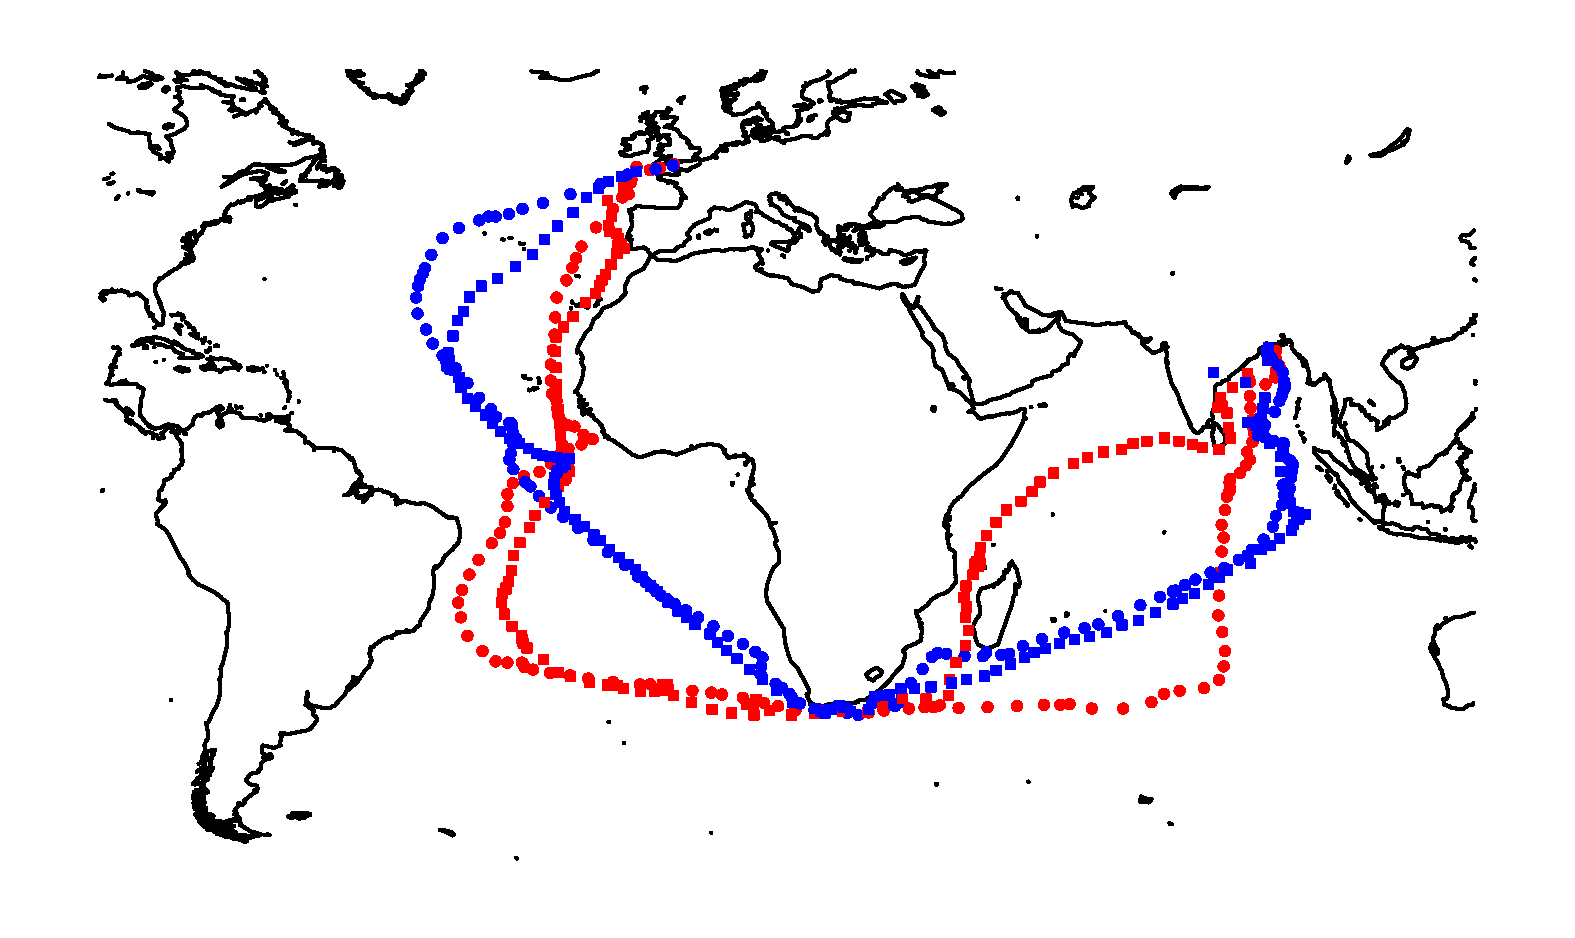
\includegraphics[angle=0, width=0.8\textwidth]{../figures/TG+A_routes.pdf}
\caption{Daily positions on the outward (red) and return (blue)voyages of the Astel in 1812-13 (squares) and Thomas Grenville in 1827-28 (circles).}
\label{Fsroc2}
\end{center}
\end{figure*}
The route back was simpler - a direct route round the Cape using the easterly trades, north-west into the mid-Atlantic and then back to England with the Northern Hemisphere westerlies.

Figure \ref{Fsroc1} shows the coverage of the observations from all 891 logs. The observations are strongly concentrated along the standard routes, but with enough variation to explore a large area of the Atlantic and Indian Oceans - occasional ships do take radically different routes - visiting the Red sea and Persian Gulf, or looping through the South Pacific on the way to Hong Kong. The records are fairly evenly distributed through time, with at least 30 ships contributing in every year between 1794 and 1833.
\begin{figure*}[!hbp]
\begin{center}
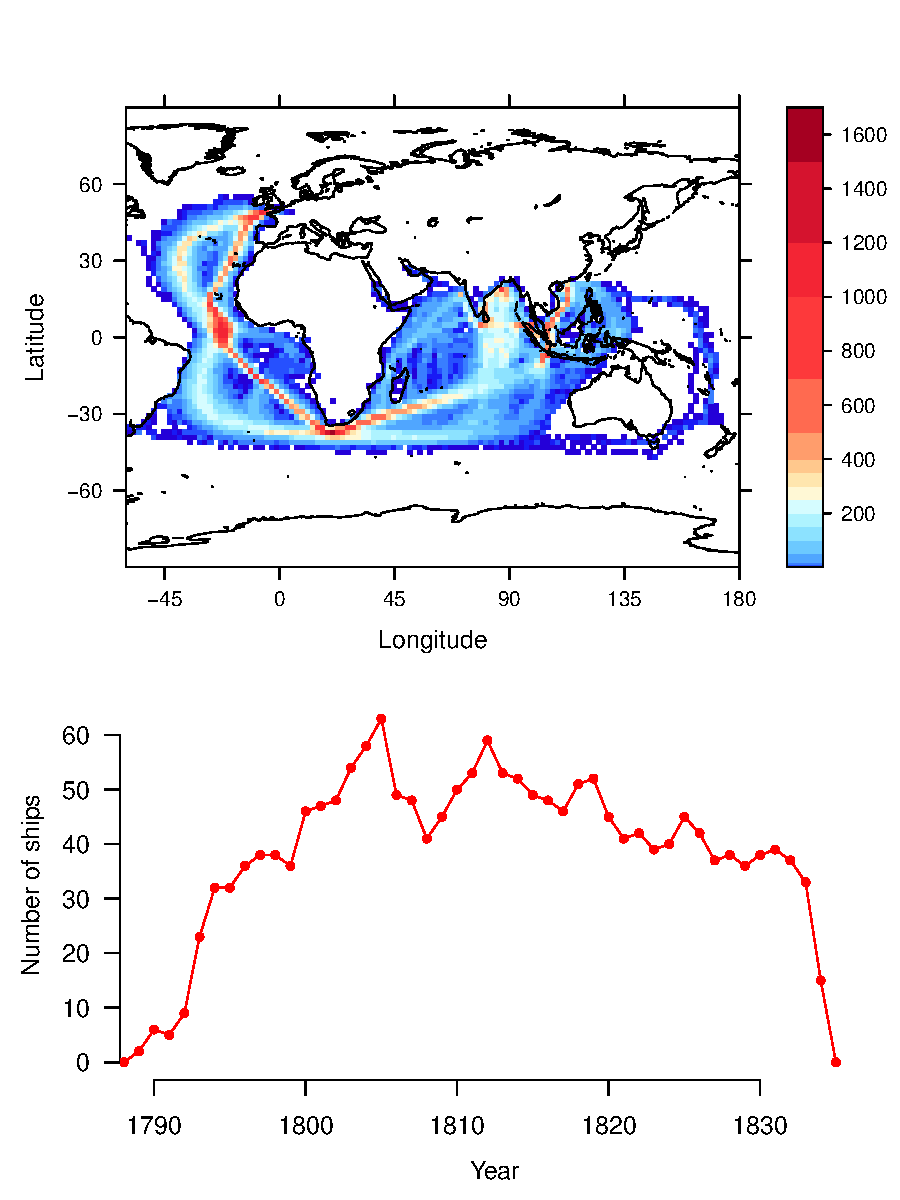
\includegraphics[angle=0, width=0.8\textwidth]{../figures/coverage}
\caption{Geographical coverage of the observations. Upper panel: total number of observations in each 2x2 degree square. Lower panel: number of ships providing observations in each year.}
\label{Fsroc1}
\end{center}
\end{figure*}

\section{Temperature, pressure and wind}

The logbooks contain instrumental observations of air pressure and temperature, and qualitative descriptions of wind speed. The details of how the measurements were made is not known, and we should expect some biases even in the instrumental observations, caused by limitations in the instruments used and the observational protocols. The model and make of instruments used on board the EEIC vessels is rarely recorded within the logbooks, and in most cases no record has been found indicating the manufacturer or type of instrument used. Dalrymple's 1775 voyages used barometers and thermometers of Nairne and Blunt manufacture \citep{Dalrymple78} but it is known from some of the more assiduously maintained logbooks that barometers of different manufacture were also used, such as Dolland, Barraud, Troughton, and Gilbert. On occasion more than one barometer was in use (e.g. Dolland, Barraud and Troughton on board the Thomas Coutts voyage of 1817-1819), and multiple thermometers are also occasionaly seen (e.g. Gilbert and Blunt manufactures on board the Neptune voyage of 1814-15). It is likely that a diverse range of instruments was used across the EEIC fleet.

 The vast majority of the temperature and pressure observations were made at noon (a handfull of logbooks record morning and afternoon observations on the same day); the location of the instruments is not known for certain, but it is likely that the thermometer and barometer were kept together in the captain's quarters and adjacent gallery at the stern of the vessel --- Dalrymple's report includes the following ``this thermometer belonged to Mr. Russell, and hung in the open air in the balcony'' \citep{Dalrymple78}.

\subsection{Temperature}

The temperatures are recorded in degrees Fahrenheit: usually to a precision of 1 degree but sometimes to a quarter or a tenth of a degree. In some instances, thermometer values were recorded in the format of degrees and seconds (e.g. $82^\circ 45'$, representing $82.75^\circ F$, as seen in figure \ref{Ftl1}), similar to the typical format for latitude or longitude. As the observations predate the development of the modern Stevenson-type screen, the major difficulty in comparing them to modern observations will be their exposure - the details of how the thermometer was screened from solar radiation. It is likely that the thermometers were kept in the stern galley of the ships and that they were less well screened than the modern standard, and also contaminated by ship heating \citep{chenoweth00homogenization,Berry05}. They will therefore be biased warm, and the bias will be larger in regions where the surface solar radiation is large. Figure \ref{pwat1} shows the distribution of the temperature anomalies (difference from recent values).
\begin{figure*}[!hbp]
\begin{center}
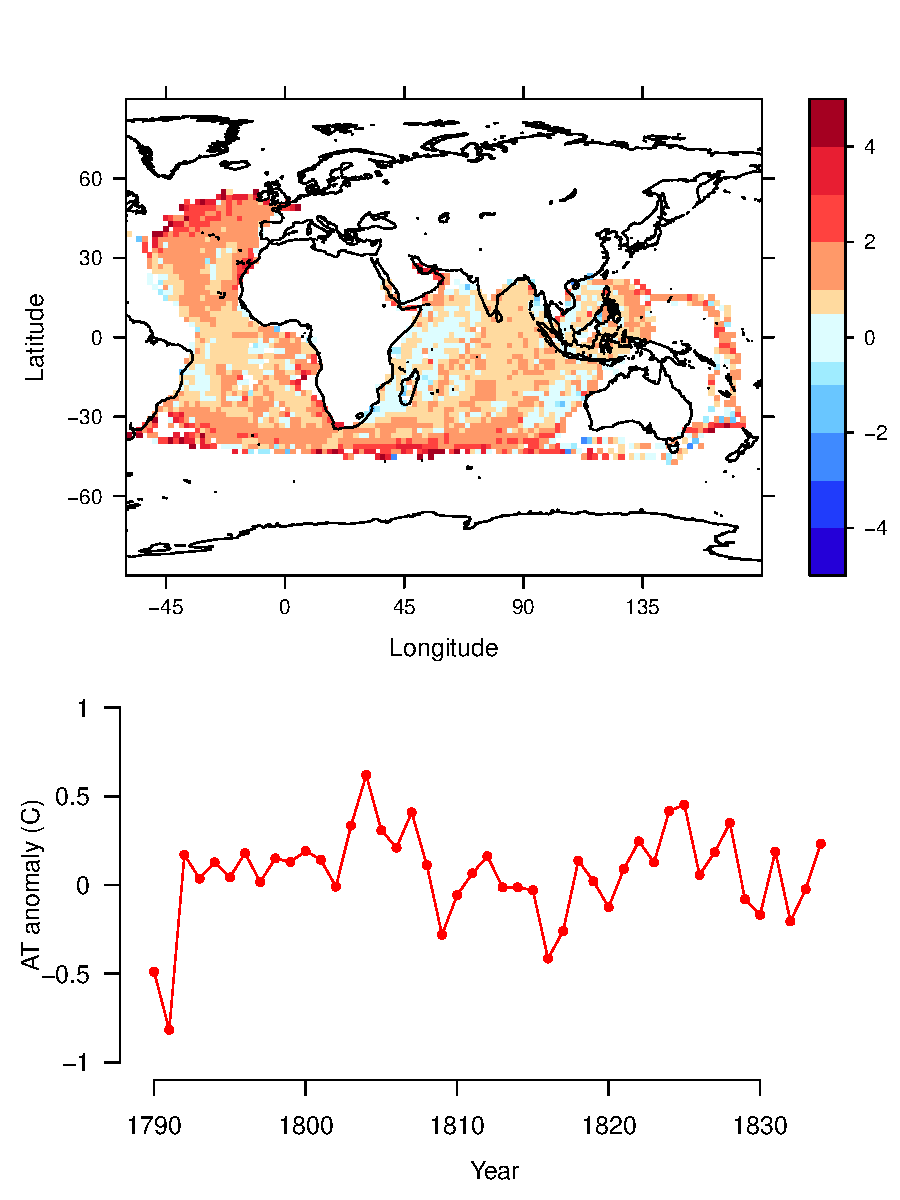
\includegraphics[angle=0, width=0.8\textwidth]{../figures/temperatures}
\caption{Air temperature (AT) anomalies: observations minus an air-temperature climatology for 1961--90 \citep{rayner03HadISST1}. Upper panel: truncated mean AT anomaly in each 2x2 degree square. Lower panel: truncated mean AT anomaly in each year.}
\label{pwat1}
\end{center}
\end{figure*}
The temperatures are consistently warmer than their recent equivalents, but the difference is much more likely to be a result of exposure bias than an indication that surface temperatures were warmer in 1789-1834 than in 1961-90. The mean temperature changes little over the period of the observations, with modest falls in 1809 and 1816 --- almost certainly a consequences of the two large tropical volcanic eruptions in the period.

\subsection{Pressure}

The pressures were recorded in inches of mercury, usually to a decimal precision of $1/100$ of an inch, but occasionally as a fraction (e.g. $29 {7\over8}"$). The pressures have been corrected for gravity (using the observed ship latitude) and for temperature (using the associated air temperature where available - no barometer attached temperatures were recorded). Figure \ref{pwat2} shows the distribution of the pressure anomalies (difference from recent values).
\begin{figure*}[!hbp]
\begin{center}
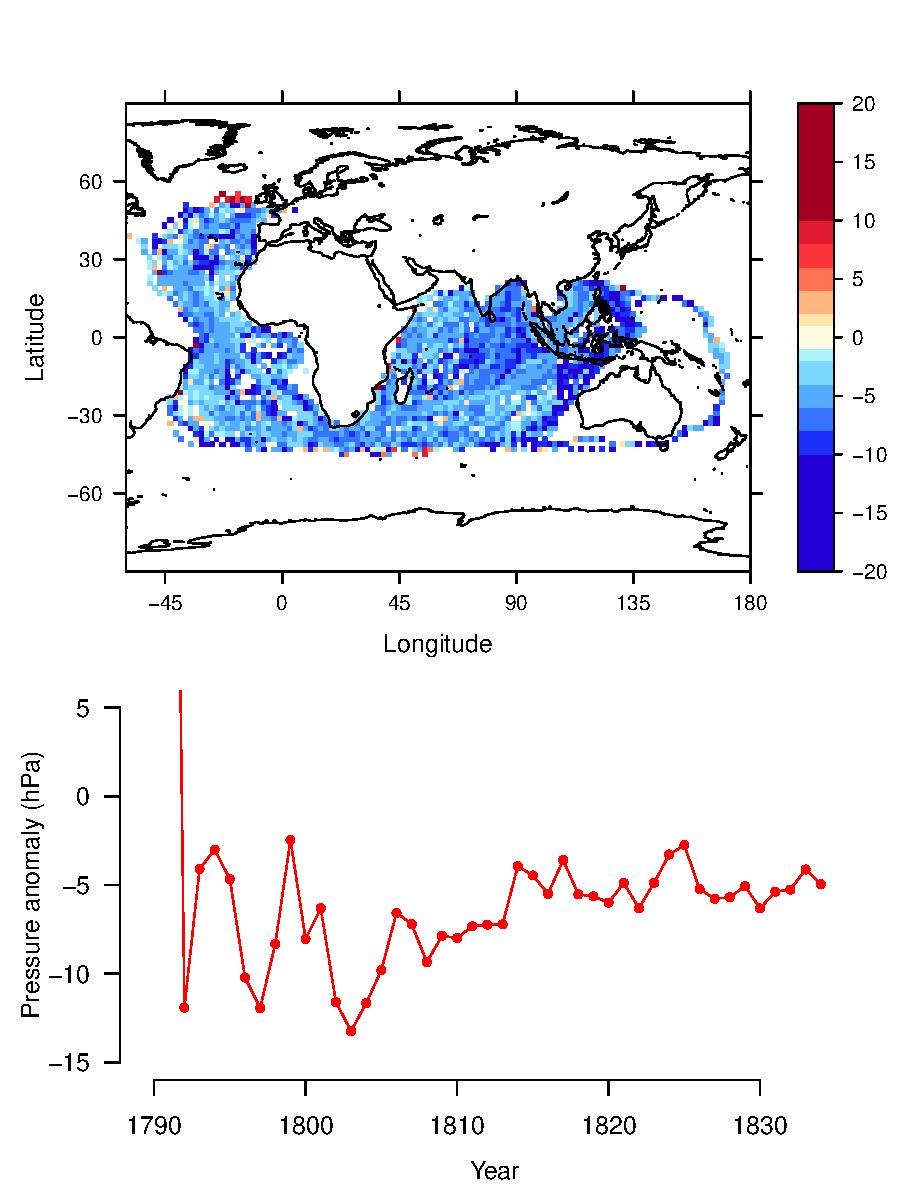
\includegraphics[angle=0, width=0.8\textwidth]{../figures/pressures}
\caption{Air Pressure (AP) anomalies: observations minus a sea-level pressure climatology for 1961--90 \citep{allan06meansealevelpressure}. Upper panel: mean AP anomaly in each 2x2 degree square. Lower panel: mean AP anomaly in each year.}
\label{pwat2}
\end{center}
\end{figure*}
The pressures are systematically and consistently about $5hPa$ (0.15 inches) below their recent equivalents. This bias has been observed before in pre-1855 marine observations \citep{ansell06emulate,brohan10corral} and the cause is still unknown. It is unlikely to be an effect of gravity or temperature correction because it doesn't vary with temperature or latitude, and it seems equally unlikely to be an artifact of the movement of the ship as it appears equally in stormy and calm regions.

 However, in 1818, Alexander Adie patented the sympiesometer, a mercury-less marine barometer containing coloured almond oil and hydrogen gas \citep{middleton64}. Several of the later EEIC voyages carried a sympiesometer, either in tandem with the mercury barometer or as a standalone pressure gauge: 31 of the 893 digitized logbooks have records from sympiesometers. Of those 31 logs, 30 also contained records from a mercury barometer, and in some cases simultanious observations from both instruments were recorded. Figure \ref{ps1} compares the simultanious barometer and sympiesometer readings for the ships providing such comparisons. 
\begin{figure*}[!hbp]
\begin{center}
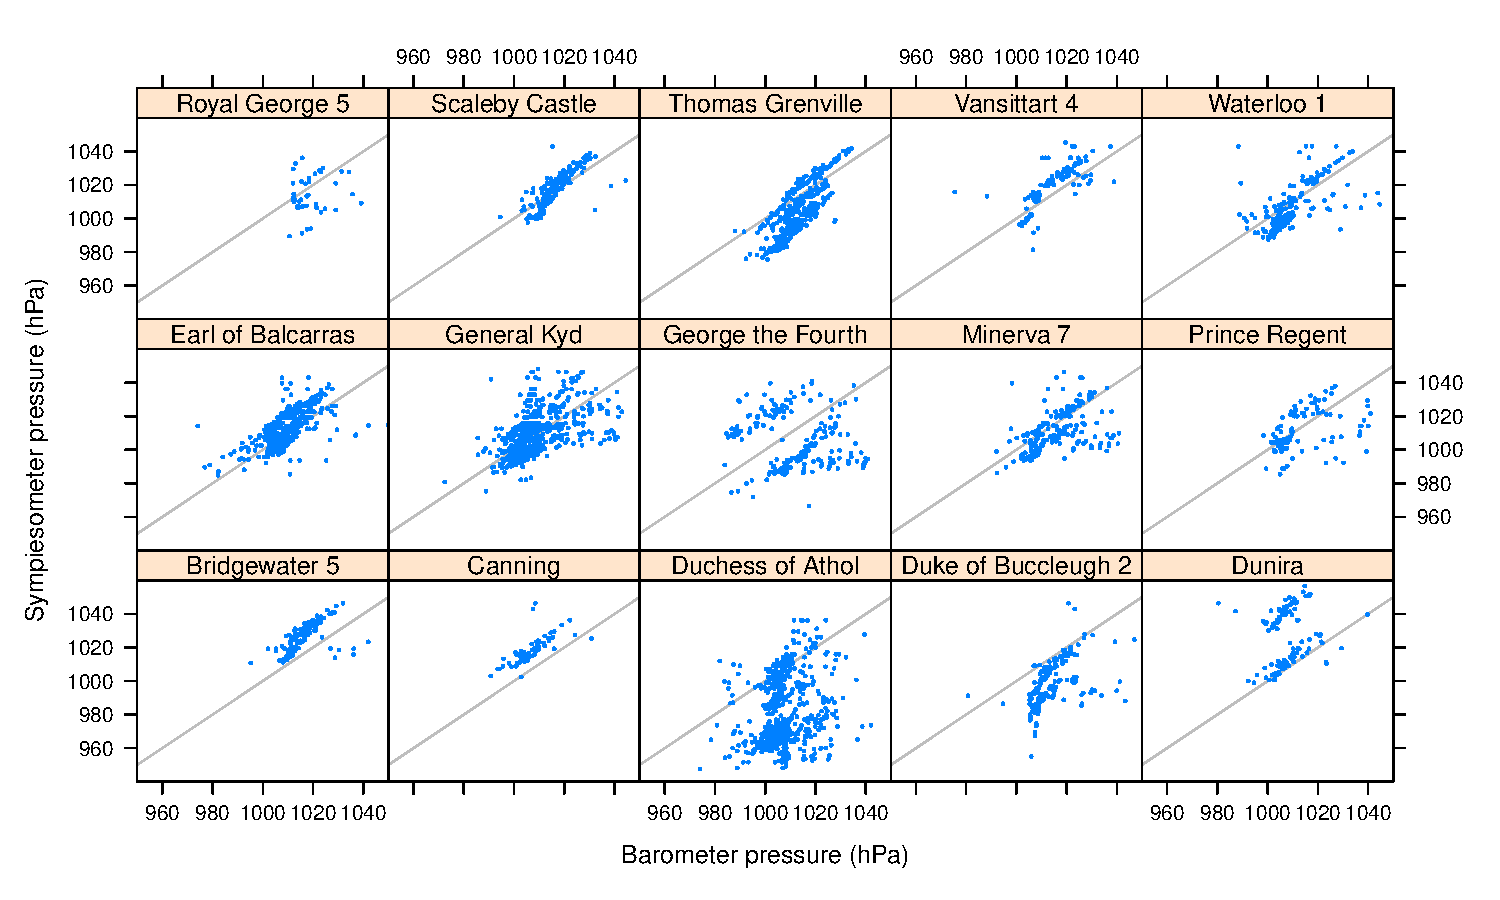
\includegraphics[angle=0, width=0.8\textwidth]{./../../../analysis/sympiesometer/sym_v_pre_censored.pdf}
\caption{Simultanious pressure and sympiesometer readings from the 15 ships that recorded observations from both instruments on the same day. Both instruments gave readings in inches, and they have been converted to hPa in the same way, except that the barometer readings have been corrected for temperature and gravity, and the sympiesometer readings have not, as such corrections are not appropiate for sympiesometers. The grey lines mark the 1:1 relationship (sympiesometer=barometer).}
\label{ps1}
\end{center}
\end{figure*}

These early sympiesometer measurements are not encouraging, as there are large and systematic differences between the sympiesometer and barometer measurements. The sympiesometer was designed to be portable and to respond rapidly to pressure changes, rather than for accuracy and stability; and time-series of sympiesometer measurements (not shown) often show large drifts in pressure readings over a voyage. So the indications are that sympiesometer records will need close attention to calibration and correction in order to be useful for historical reconstructions.

The pressure observations included in the attached IMMA records are believed to be from mercury barometers, but it is possible that in some of the later voyages the pressure observations are actually from a sympiesometer. That is, a sympiesometer has been used in place of the usual mercury barometer but the substitution is not mentioned in the logbook.

\subsection{Wind speed}

The wind speed observations in the logbooks are, as is usual at sea, subjective assessments based on the sails carried and the state of the sea. The vocabulary of such assessments was not formally standardised until the 1830s, when Sir Francis Beaufort succeeded in introducing an official scale, but, even in this pre Beaufort-scale age, sailors were very consistent in their description of the winds, and it is possible to make quantitative estimates of the wind speed from the language in the logs \citep{cliwoc03dictionary}. Figure \ref{pwat4} shows the most frequent wind-force terms used and their Beaufort equivalents where available.
\begin{figure*}[!hbp]
\begin{center}
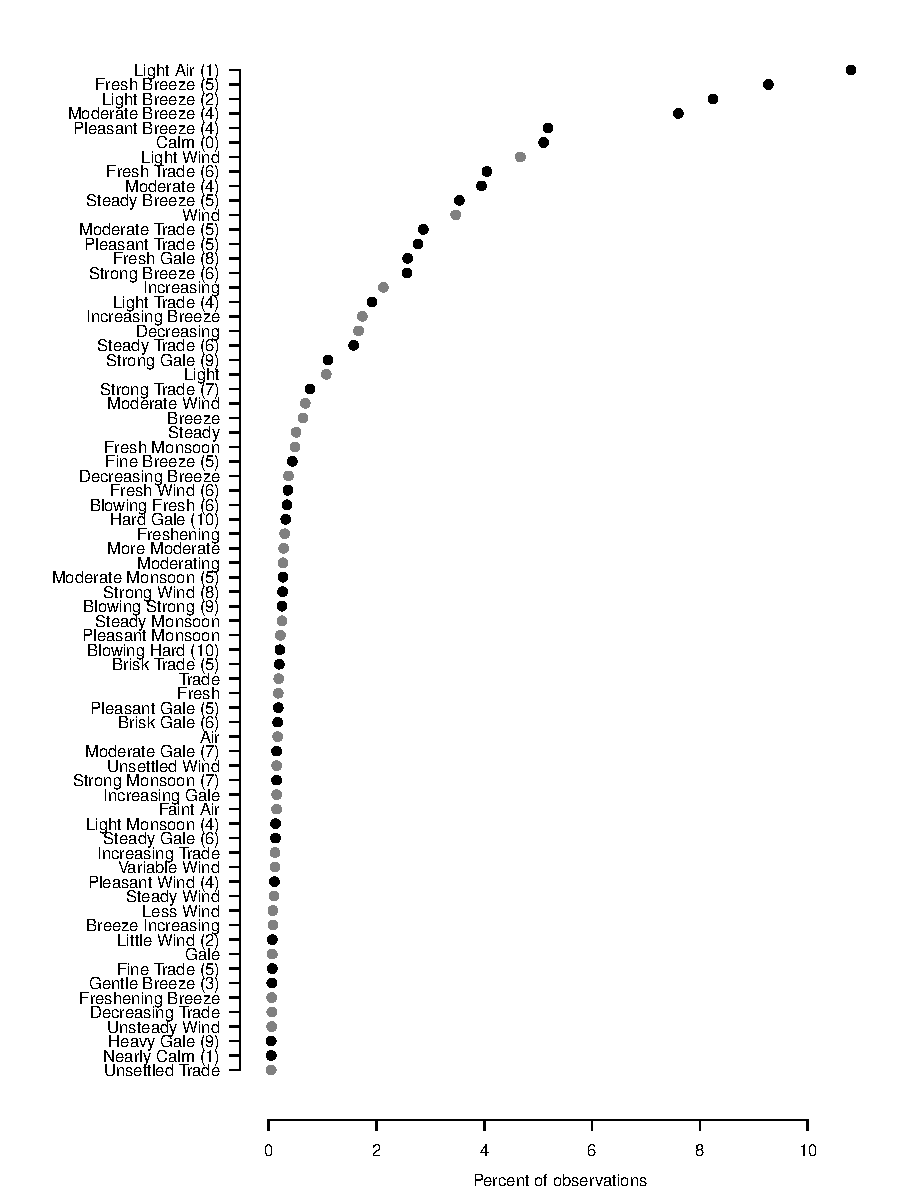
\includegraphics[angle=0, width=0.8\textwidth]{../figures/wind_term_frequencies}
\caption{The most common wind-force descriptors in the logs. Black points mark descriptors that can be converted to a Beaufort force using the CLIWOC dictionary (the Beaufort category is given in brackets after the descriptor in these cases). Grey points are terms which can't be converted.}
\label{pwat4}
\end{center}
\end{figure*}

About 80\% of the terms encountered can be converted to Beaufort forces, and so to 10-metre wind speeds in $m/s$. Figure \ref{pwat3} shows the distribution of the inferred wind-speed anomalies (difference from recent values).
\begin{figure*}[!hbp]
\begin{center}
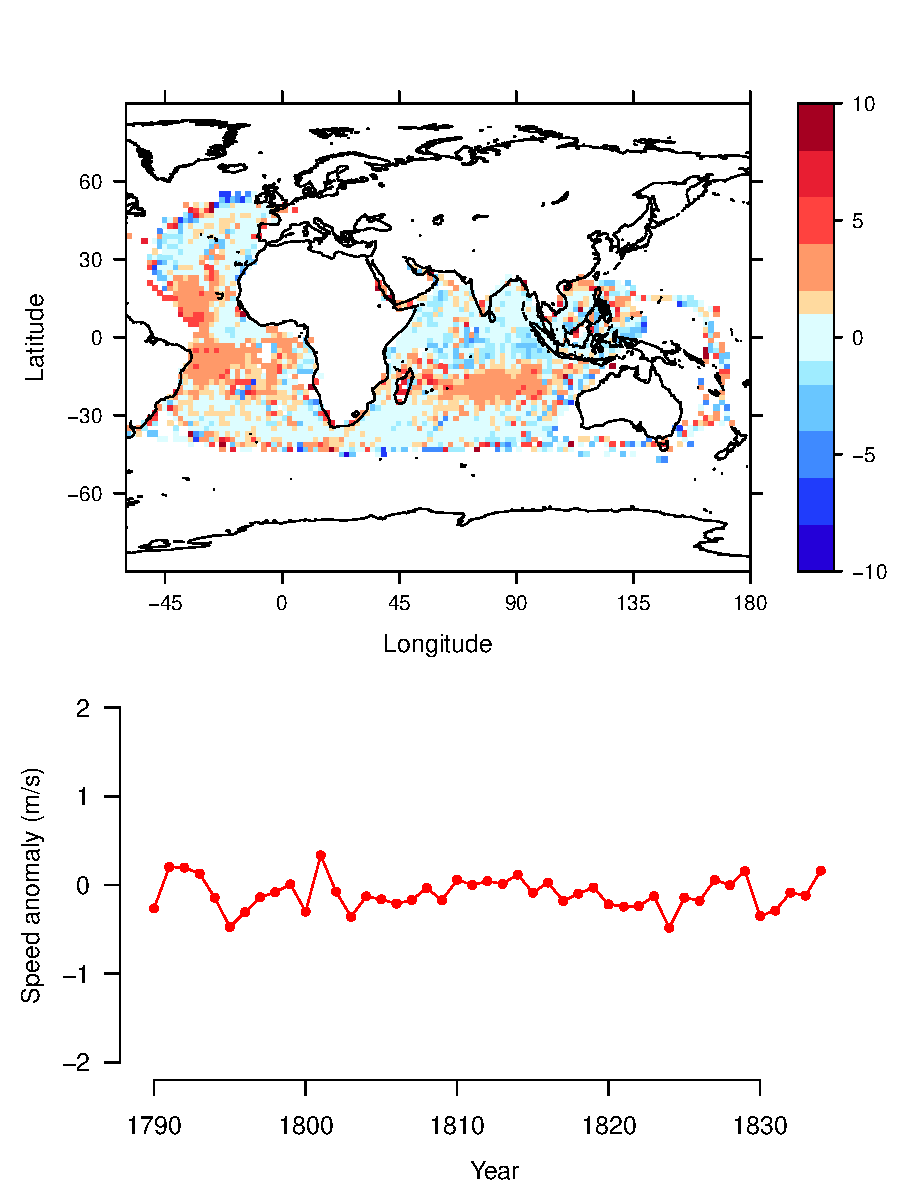
\includegraphics[angle=0, width=0.8\textwidth]{../figures/wind_speeds}
\caption{Wind Speed (WS) anomalies: observations minus a wind-speed climatology for 1961--90 from the ERA-40 reanalysis \citep{uppala05reanalysis}. Upper panel: truncated mean WS anomaly in each 2x2 degree square. Lower panel: truncated mean WS anomaly in each year.}
\label{pwat3}
\end{center}
\end{figure*}
The notable feature of figure \ref{pwat3} is the large anomalies in the trade-wind regions. It's possible that the trade winds were stronger around 1800, but as no equivalent anomaly appears in the pressure fields it's more likely that the CLIWOC dictionary is slightly mis-calibrated in those regions (stronger trades imply a stronger sub-tropical high or a deeper equatorial low).

Although all the pressure and temperature observations in the selected logbooks were digitised, budget constraints meant that not all of the much more numerous and various wind observations were. There are also wind observations in the more than 3000 logbooks in the BL archive that were not examined in this study (because they had no instrumental pressure or temperature observations). So much more information on wind fields is still potentially available in the BL EEIC logbook archive. If extracted in a future project, these records would provide information on sub-daily weather variability back into the $17^{th}$ century.

\section{The Pacific fleet of 1805}

In 1804 a fleet of East Indiamen coming back from China were attacked by a French squadron under the command of Admiral Linois. Despite having no warship escorts, the fleet managed to beat off the attack (the famous battle of Pulo Aura) documented in many EEIC logbooks \citep{rodger04}, but the conventional route to China through the Sunda Strait clearly left the ships vulnerable to capture. To avoid this risk {\bf[Refs.]}, a fleet of ships setting out the following year took an alternative route to Hong Kong - staying in the southern westerlies until east of Australia, and then looping up through the south Pacific. Five ships from this fleet are included in the digitised logbooks (Alnwick Castle, Arniston, Ceres 4, Cuffnells, and Royal Charlotte 5) and, as they travelled as a fleet, they are a useful set of records for inter-comparison: to see to what extent observations of the same surrounding weather differ from ship to ship. Figure \ref{pf1} shows the route taken by the fleet (they made no stops between Rio de Janeiro and Hong Kong), and figures \ref{pf2} and \ref{pf3} show the variation between reported positions and temperatures between the ships.

\begin{figure*}[!hbp]
\begin{center}
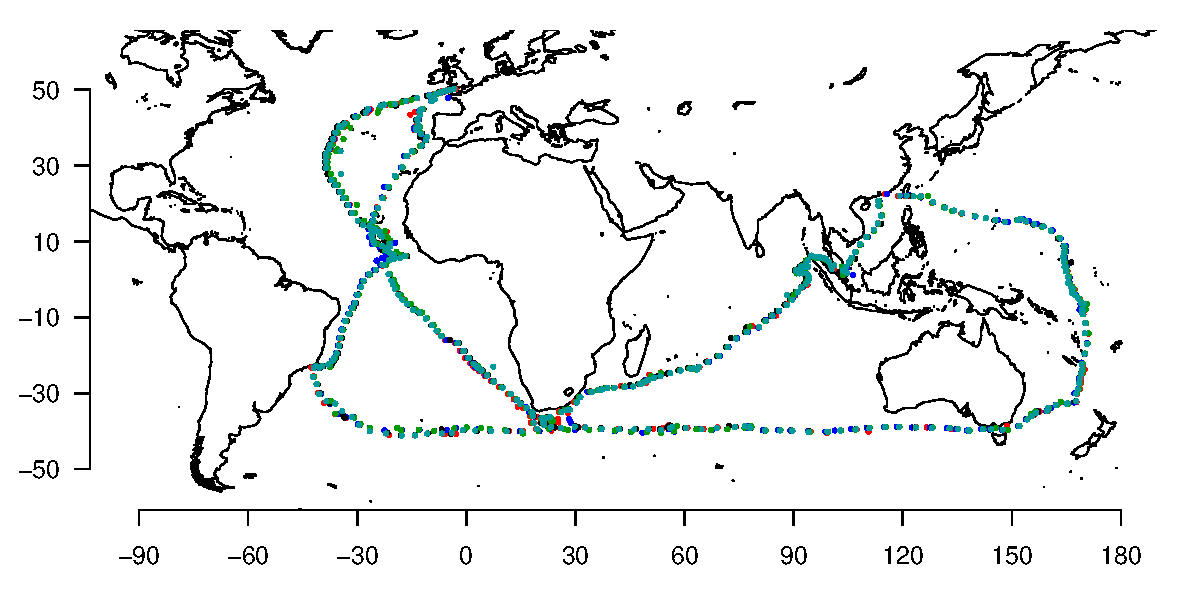
\includegraphics[angle=0, width=0.8\textwidth]{./../../../analysis/south_pacific/figures/all_route}
\caption{Daily positions from each of the China Fleet ships in 1804--5. Alnwick Castle (red), Arniston (blue), Ceres 4 (black), Cuffnells (green), and Royal Charlotte 5 (teal).}
\label{pf1}
\end{center}
\end{figure*}

\begin{figure*}[!hbp]
\begin{center}
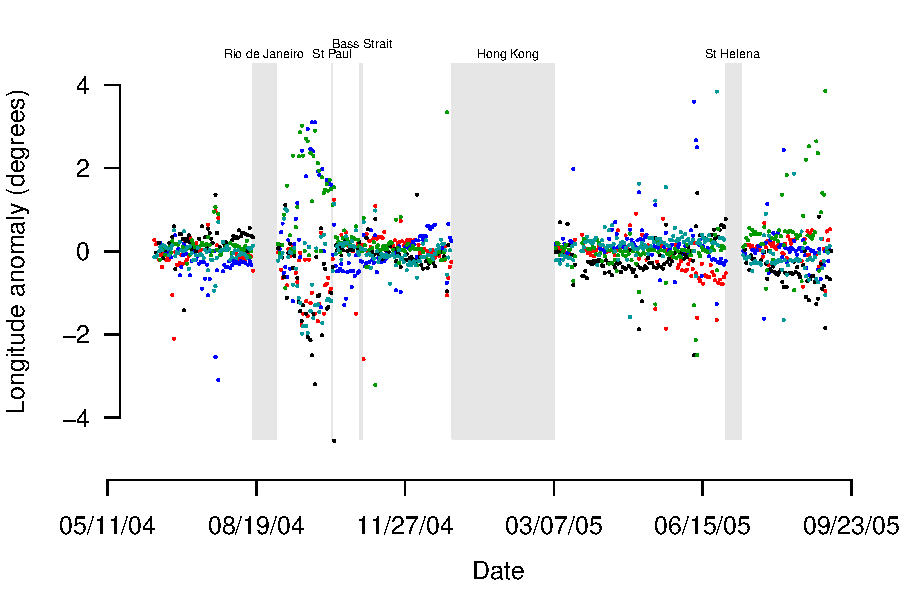
\includegraphics[angle=0, width=0.8\textwidth]{./../../../analysis/south_pacific/figures/longitude_v_time}
\caption{Longitude anomalies (ship longitudes minus the fleet mean) from each of the China Fleet ships in 1804--5. Alnwick Castle (red), Arniston (blue), Ceres 4 (black), Cuffnells (green), and Royal Charlotte 5 (teal).}
\label{pf2}
\end{center}
\end{figure*}
The logbooks contain spaces for entry of longitudes estimated both by dead reckoning and by chronometer, and in almost all cases a chronometer longitude is recorded and is the record digitised. So the very uncertain longitudes found from earlier ship records (for example by the CLIWOC project) are not a problem in this case: longitudes are recorded with respect to the Greenwich meridian and are broadly accurate. In a few cases, different meridians were used but not always disclosed. These were corrected during conversion to the IMMA format to use the Greenwich meridian. There are, however, still uncertainties in the ship positions, especially when the ships are some distance from any land which could be used for position fixes. Figure \ref{pf2} shows that relatively large differences appear between the ships' position estimates during their voyage through the South Atlantic, but these differences reduce abruptly when the ships encounter Ile St Paul, with provides them with a position fix. Latitude variations (not shown) are similar but smaller, as latitude could be observed more precisely with the technology of the time.

\begin{figure*}[!hbp]
\begin{center}
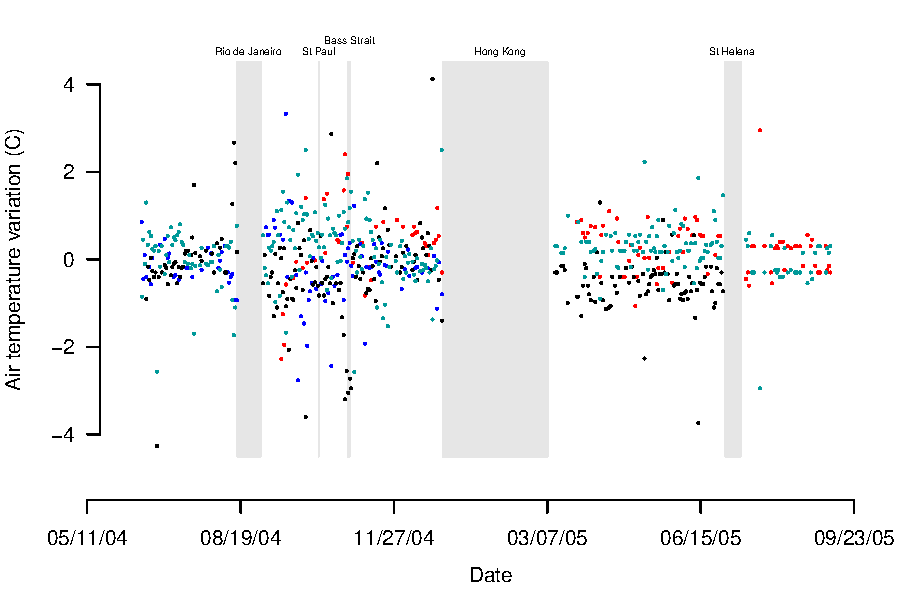
\includegraphics[angle=0, width=0.8\textwidth]{./../../../analysis/south_pacific/figures/temperature_v_time}
\caption{Temperature anomalies (ship air temperature minus the fleet mean) from each of the China Fleet ships in 1804--5. Alnwick Castle (red), Arniston (blue), Ceres 4 (black), Cuffnells (green), and Royal Charlotte 5 (teal).}
\label{pf3}
\end{center}
\end{figure*}
We expect some scatter between the temperatures observed in different ships even when sailing together: both systematic differences resulting from separate thermometers and differently exposed locations, and random variability resulting from the transiently different weather and local environments. The random variability is clearly substantial --- typically of order $1^\circ C$, but the systematic differences are much smaller --- indicating that the EIC ships were consistent in how they made their observations.

\begin{table*}[!hbp]
\begin{minipage}[b]{0.5\linewidth}\centering
{\scriptsize
\begin{tabular}{|p{3.5cm}|p{3.5cm}|}
\hline 
{\bf Ship Name} & {\bf Years of operation} \\ 
\hline
Melville Castle & 1789--1790,1792--1793,1796--1802\\
\hline
Rose (2) & 1789--1790,1799--1800\\
\hline
Barwell (1) & 1790--1791,1795--1796\\
\hline
Belvedere & 1790--1791\\
\hline
Earl Of Abergavenny (2) & 1790,1797--1800\\
\hline
Marquis Of Lansdown & 1790--1791,1793--1800\\
\hline
Ocean (1) & 1791--1797\\
\hline
Bridgewater (3) & 1791--1793,1796--1797\\
\hline
Lascelles & 1792--1796\\
\hline
Middlesex (2) & 1792--1795\\
\hline
Royal Admiral (1) & 1792--1796\\
\hline
Swallow (3) & 1792--1794\\
\hline
Ganges (1) & 1792--1795\\
\hline
General Goddard & 1792--1793\\
\hline
Pigot (2) & 1793--1794\\
\hline
Ceres (2) & 1793--1794\\
\hline
Warley (1) & 1793--1794\\
\hline
Berrington & 1793--1794\\
\hline
General Coote & 1793--1794\\
\hline
Rodney (2) & 1793--1796\\
\hline
Princess Amelia (3) & 1793--1796\\
\hline
Francis (2) & 1793--1796\\
\hline
Exeter (2) & 1793--1794,1800--1801,1803--1804,1810--1811\\
\hline
Lord Thurlow & 1793--1794,1797--1802\\
\hline
Lord Walsingham & 1793--1794,1797--1799\\
\hline
Minerva (1) & 1793--1796,1799--1800\\
\hline
Earl Of Chesterfield & 1793--1794\\
\hline
Earl Of Wycombe & 1794--1795,1797--1799\\
\hline
Sir Edward Hughes & 1794--1795,1797--1803\\
\hline
Woodford (1) & 1794--1805,1807--1808,1810--1811\\
\hline
Thetis (1) & 1794--1797\\
\hline
Rockingham (1) & 1794--1795,1798--1802\\
\hline
Walpole (4) & 1794--1795\\
\hline
Phoenix (3) & 1794--1795\\
\hline
Lord Hawkesbury & 1794--1802,1804--1806\\
\hline
Taunton Castle & 1794--1795,1799--1800,1804--1805,1809--1810\\
\hline
Europa (2) & 1794--1795\\
\hline
Queen (4) & 1794--1798\\
\hline
Carnatic (2) & 1794--1795,1801--1802\\
\hline
Princess Of Wales (3) & 1795--1797\\
\hline
Earl Of Oxford & 1795--1796\\
\hline
Cirencester & 1795--1796,1812--1813\\
\hline
London (13) & 1795--1796\\
\hline
Bellona & 1795--1798\\
\hline
Hillsborough (2) & 1795--1798\\
\hline
Kent (5) & 1795--1797\\
\hline
Woodcot & 1795--1796\\
\hline
Brunswick (1) & 1795--1797\\
\hline
Cuffnells & 1796--1800,1802--1805,1809--1810\\
\hline
Princess Charlotte (1) & 1796--1797\\
\hline
Albion (2) & 1796--1798\\
\hline
Royal Charlotte (5) & 1796--1807,1809--1815\\
\hline
Essex (4) & 1796--1798\\
\hline
True Briton (4) & 1796--1798,1801--1802\\
\hline
Airly Castle & 1796--1797,1804--1806\\
\hline
Walmer Castle & 1796--1798,1802--1805,1815--1816\\
\hline
Boddam & 1796--1800\\
\hline
Manship (1) & 1796--1800\\
\hline
Good Hope (3) & 1796--1799\\
\hline
Henry Addington (1) & 1796--1798\\
\hline
Ganges (3) & 1797--1802\\
\hline
Prince William Henry & 1797--1799\\
\hline
Britannia (4) & 1797--1805\\
\hline
Warley (2) & 1797--1800,1805--1809,1811--1814\\
\hline
Hope (2) & 1797--1808,1811--1816\\
\hline
Arniston & 1797--1798,1804--1807,1810--1811\\
\hline
Eurydice & 1797--1799\\
\hline
Sulivan & 1797--1798\\
\hline
Osterley (3) & 1798--1800\\
\hline
\end{tabular}
}
\end{minipage}
\hspace{0.5cm}
\begin{minipage}[b]{0.5\linewidth}
\centering
{\scriptsize
\begin{tabular}{|p{3.5cm}|p{3.5cm}|}
\hline 
{\bf Ship Name} & {\bf Years of operation} \\ 
\hline
Earl Howe & 1798--1810\\
\hline
Lord Duncan & 1798--1806\\
\hline
Ocean (3) & 1798--1800\\
\hline
Tellicherry & 1798--1799\\
\hline
Earl Cornwallis & 1798--1800\\
\hline
Orpheus & 1798--1800\\
\hline
Charlton & 1799--1806\\
\hline
Asia (4) & 1799--1803\\
\hline
Hindostan (2) & 1799--1800\\
\hline
Duke Of Buccleugh (1) & 1799--1800\\
\hline
Preston & 1799--1800\\
\hline
Herculean & 1800--1801\\
\hline
Dorsetshire & 1800--1801,1803--1804,1806,1811--1812,1814--1815,1817--1818,1820--1823\\
\hline
Earl Spencer (2) & 1800--1801,1803--1810\\
\hline
Neptune (5) & 1800--1801,1804--1807,1809--1810,1812--1815\\
\hline
Hugh Inglis & 1800--1801,1810--1812\\
\hline
Lady Burges & 1800--1805\\
\hline
Walthamstow & 1800--1801,1804--1805,1808--1813\\
\hline
Lord Nelson & 1800--1801,1806--1807\\
\hline
Ceres (4) & 1800--1805,1808--1809\\
\hline
City Of London & 1800--1801,1803--1808,1812--1813\\
\hline
Bengal & 1800--1802,1806--1807\\
\hline
Canton & 1800--1805,1808--1811\\
\hline
Georgiana (1) & 1800--1803,1805--1807\\
\hline
Hawke (5) & 1800--1801\\
\hline
Earl St & 1800--1801,1808--1813\\
\hline
Henry Dundas & 1801--1802\\
\hline
Calcutta (4) & 1801--1804\\
\hline
Alfred (2) & 1801--1802,1807--1808,1810--1811\\
\hline
Caledonian (2) & 1801--1803\\
\hline
Henry Addington (2) & 1801--1802,1805--1806,1811--1812,1814--1815\\
\hline
Walpole (5) & 1801--1802\\
\hline
Ocean (4) & 1801--1803,1805--1806,1808--1809\\
\hline
Northampton (2) & 1801--1805,1807--1810,1818--1819\\
\hline
Princess Mary (2) & 1801--1805\\
\hline
Fort William (2) & 1801--1802\\
\hline
Monarch & 1801--1802\\
\hline
Experiment (2) & 1801\\
\hline
Manship (2) & 1801--1803\\
\hline
Sarah Christiana & 1801--1802\\
\hline
Comet (2) & 1801--1803\\
\hline
Marquis Of Ely & 1802--1805,1811--1814,1819--1820\\
\hline
Marquis Wellesley & 1802--1803,1806--1808\\
\hline
Castle Eden & 1802--1804\\
\hline
Lady Jane Dundas & 1802--1807\\
\hline
Thames (2) & 1802--1805,1809--1810,1812--1813\\
\hline
Sir William Bensley & 1802--1811\\
\hline
Tottenham & 1802--1803,1806--1810\\
\hline
Travers & 1802--1806\\
\hline
Alnwick Castle & 1802--1813,1815--1816\\
\hline
Marchioness Of Exeter & 1802--1803,1811--1814,1816--1817\\
\hline
Devaynes & 1802--1808,1811--1812\\
\hline
Ann (1) & 1803--1809,1814--1815\\
\hline
Experiment (4) & 1803--1805\\
\hline
Cumberland & 1803--1804,1809--1810\\
\hline
Warren Hastings (2) & 1803--1804\\
\hline
Harriet (3) & 1803--1811\\
\hline
Elphinstone & 1803--1811\\
\hline
Tigris (2) & 1803--1805,1810--1815\\
\hline
Marquis Cornwallis (2) & 1803\\
\hline
Windham (2) & 1803--1806,1816--1817\\
\hline
Europe (2) & 1803--1807\\
\hline
Euphrates & 1803--1805\\
\hline
General Stuart & 1803--1804,1807,1811--1814\\
\hline
Essex (5) & 1803--1805,1808--1809,1819--1820\\
\hline
Carmarthen & 1803--1818\\
\hline
Union (4) & 1803--1804,1808--1812,1815--1818\\
\hline
\end{tabular}
}
\end{minipage}
\vspace{0.5cm}
\caption{Ships from which observations were taken (1 of 2 --- starting dates 1789 to 1803).}
\label{T1.1}
\end{table*}

\begin{table*}[!hbp]
\begin{minipage}[b]{0.5\linewidth}\centering
{\scriptsize
\begin{tabular}{|p{3.5cm}|p{3.5cm}|}
\hline 
{\bf Ship Name} & {\bf Years of operation} \\ 
\hline
Ocean (5) & 1803--1805\\
\hline
Lord Melville (1) & 1803--1808,1811--1816\\
\hline
Dover Castle & 1804--1805,1809--1810\\
\hline
Indus & 1804--1805,1810--1815\\
\hline
Alexander (3) & 1804--1809,1814\\
\hline
Lord Eldon & 1804--1814\\
\hline
Waller & 1804\\
\hline
Winchelsea (3) & 1804--1807,1810--1815,1817--1818,1820--1823,1831--1832\\
\hline
Ocean (6) & 1804--1814\\
\hline
Huddart & 1804--1805,1808--1809,1815--1816\\
\hline
United Kingdom & 1804--1805,1807--1808\\
\hline
Bombay Castle & 1805--1806\\
\hline
Surrey (1) & 1805--1810\\
\hline
Northumberland (5) & 1805--1818\\
\hline
Royal George (4) & 1805--1811,1814--1818\\
\hline
Sir William Pultney & 1805--1807,1815--1816\\
\hline
Streatham (4) & 1805--1814,1817--1818\\
\hline
Glory & 1805--1807\\
\hline
William Pitt (2) & 1805--1807,1810--1820\\
\hline
Phoenix (5) & 1805--1809,1816--1819\\
\hline
Wexford & 1805--1817\\
\hline
David Scott (2) & 1806--1807,1812--1813,1815--1816\\
\hline
Glatton (4) & 1806--1807,1809--1810,1812--1815\\
\hline
Sir Stephen Lushington & 1806--1811\\
\hline
Regent & 1807,1816--1819,1822\\
\hline
Lady Castlereagh & 1807--1817\\
\hline
Admiral Gardner & 1807--1808\\
\hline
Union (5) & 1807--1808,1813--1814\\
\hline
Lord Keith & 1808--1811,1814--1819\\
\hline
Princess Amelia (4) & 1809--1825\\
\hline
Thomas Grenville & 1809--1832\\
\hline
Warren Hastings (3) & 1809--1810,1814--1821,1825--1828,1831--1834\\
\hline
Coutts & 1809--1810,1812--1815\\
\hline
Lady Lushington & 1809--1814,1818--1819\\
\hline
Farlie & 1809--1814,1818--1819\\
\hline
Charles Grant & 1810--1816,1819--1830,1832--1833\\
\hline
Surat Castle (2) & 1810--1815\\
\hline
Lady Carrington & 1810,1812--1817\\
\hline
Midas & 1810--1811\\
\hline
Warren Hastings (5) & 1811--1812,1815--1816,1819--1820,1823--1826\\
\hline
Carnatic (3) & 1811--1820\\
\hline
John Palmer & 1811\\
\hline
Cambridge & 1811--1812,1825--1827\\
\hline
Scaleby Castle & 1811--1812,1814--1828,1831--1834\\
\hline
William Pitt (3) & 1811--1812\\
\hline
Harleston & 1811--1812\\
\hline
Moffat & 1811--1812,1818--1819\\
\hline
Rose (4) & 1811--1822,1824--1827,1833--1834\\
\hline
General Harris & 1812--1831\\
\hline
Broxbornebury & 1812--1813,1825--1828\\
\hline
Asia (6) & 1812--1826,1832--1833\\
\hline
Marquis Of Huntley & 1812--1813,1818--1823,1831--1834\\
\hline
Perseverance (2) & 1812--1814,1818--1819\\
\hline
Marquis Camden & 1812--1814,1821--1829,1832--1833\\
\hline
Juliana & 1812--1813\\
\hline
Astell & 1812--1813,1818--1821,1824--1825,1830--1831\\
\hline
Princess Charlotte Of Wales & 1812--1822,1825--1828\\
\hline
Coldstream & 1812--1813,1816--1817,1822--1823\\
\hline
Cabalva & 1812--1817\\
\hline
David Scott (1) & 1813--1814\\
\hline
Marquis Of Wellington (1) & 1813--1822,1827,1829--1830\\
\hline
Atlas (4) & 1813--1830\\
\hline
\end{tabular}
}
\end{minipage}
\hspace{0.5cm}
\begin{minipage}[b]{0.5\linewidth}
\centering
{\scriptsize
\begin{tabular}{|p{3.5cm}|p{3.5cm}|}
\hline 
{\bf Ship Name} & {\bf Years of operation} \\ 
\hline
Lowther Castle & 1813--1828,1831--1834\\
\hline
Bombay & 1814--1815,1817--1822,1825--1828,1831--1834\\
\hline
Prince Regent & 1814--1815,1818--1829,1833--1834\\
\hline
Lady Melville & 1814--1821,1824--1827,1829--1834\\
\hline
Minerva (7) & 1815--1822,1825--1832\\
\hline
Surrey (2) & 1815\\
\hline
General Kyd & 1815--1816,1823--1832\\
\hline
James Sibbald & 1815--1816,1826--1829\\
\hline
Sovereign (2) & 1816--1817\\
\hline
Northampton (3) & 1816\\
\hline
Fort William (3) & 1816--1817\\
\hline
Mangles & 1816--1819\\
\hline
Buckinghamshire & 1816--1824\\
\hline
Providence (1) & 1816--1817\\
\hline
Larkins (1) & 1816--1817\\
\hline
Earl Of Balcarras & 1816--1833\\
\hline
Vansittart (4) & 1817--1824,1827--1834\\
\hline
Lord Castlereagh (1) & 1817--1820\\
\hline
Waterloo (1) & 1817--1832\\
\hline
Bridgewater (5) & 1817--1830\\
\hline
Herefordshire & 1817--1818,1821--1826,1829--1834\\
\hline
Barkworth & 1817--1818\\
\hline
Castle Huntley & 1818--1821,1824--1825,1828--1831,1833--1834\\
\hline
General Hewett & 1818--1825\\
\hline
London (14) & 1818--1823,1826--1833\\
\hline
Canning & 1818--1832\\
\hline
Duke Of York (2) & 1818--1826,1829--1830\\
\hline
Dunira & 1818--1819,1822--1823,1830--1833\\
\hline
Thomas Coutts & 1818--1825,1828--1833\\
\hline
Henry Porcher & 1818--1819\\
\hline
Matilda & 1819--1820\\
\hline
Kellie Castle & 1819--1830,1833--1834\\
\hline
Inglis & 1819--1832\\
\hline
Thames (5) & 1819--1821,1824--1827,1829--1834\\
\hline
Cornwall & 1819--1820,1826\\
\hline
Windsor (2) & 1819--1820,1825--1828,1832--1833\\
\hline
Marchioness Of Ely & 1820--1821,1826--1829\\
\hline
Orwell & 1820--1831\\
\hline
Kent (7) & 1821--1824\\
\hline
Royal George (5) & 1821--1824\\
\hline
Farquharson & 1821--1828,1831--1834\\
\hline
William Fairlie & 1822--1833\\
\hline
Berwickshire & 1822--1833\\
\hline
Sir David Scott & 1822--1825,1830--1833\\
\hline
Duchess Of Athol & 1822--1826,1828--1833\\
\hline
Repulse & 1823--1830\\
\hline
Claudine & 1824--1825\\
\hline
Macqueen & 1824--1825,1830--1833\\
\hline
Java & 1825\\
\hline
Clyde (2) & 1825--1826\\
\hline
George The Fourth & 1826--1833\\
\hline
Edinburgh & 1826--1831\\
\hline
Reliance & 1828--1833\\
\hline
Abercrombie Robinson & 1828--1833\\
\hline
Maitland & 1828--1829\\
\hline
Asia (10) & 1829--1830\\
\hline
Susan (2) & 1830--1831\\
\hline
Marquis Of Hastings & 1830--1831\\
\hline
Lord Lowther & 1830--1833\\
\hline
Duke Of Sussex & 1831--1832\\
\hline
Duke Of Buccleugh (2) & 1831--1832\\
\hline
Bencoolen & 1832--1833\\
\hline
Sherborne (2) & 1833--1834\\
\hline
\end{tabular}
}
\end{minipage}
\vspace{0.5cm}
\caption{Ships from which observations were taken (2 of 2 --- starting dates 1803 to 1833).}
\label{T1.2}
\end{table*}


\conclusions

The records of the English East India Company (EEIC), archived in the British Library, offer a remarkable new insight into the weather and climate of the late eighteenth and early nineteenth centuries. Their archives include 891 ships' logbooks containing daily temperature and pressure measurements, and wind-speed estimates, each covering a voyage from England to India or China and back. The 287,000 new weather observations extracted from those logs provide material for detailed reconstructions of the weather and climate between 1789 and 1834 and offer new insights into pre-industrial climate variability

For all three meteorological variables studied (temperature, pressure and wind) it's clear that the data can be used for investigating variability over the period of measurement, but comparison with measurements made decades or centuries later will require close attention to observational biases. Space allows only the most cursory look at the results --- more detailed investigation will follow in future analyses. The new data are attached to this paper as supplementary information, and will be submitted to the International Comprehensive Ocean-Atmosphere Dataset (ICOADS) for general use.

\begin{acknowledgement}
This work was made possible by the UK Department of Food, Energy and Rural Affairs (Defra), which paid for the investigation and photography of the original log-books; and by the US Climate Database Modernisation Program (CDMP) which transcribed the weather records from the photographs. PB was also supported by the Joint DECC and Defra Integrated Climate Programme, DECC/Defra (GA01101). 
\end{acknowledgement}

\bibliographystyle{copernicus}
\bibliography{database,bibliography_extra}

\end{document}
